% Memoria de la práctica final de PLN 2026/27 · Asistente de agenda en lenguaje natural
% Compilar desde la carpeta memoria/:  pdflatex memoria.tex  (dos veces, para referencias)
% Las figuras se leen de ../resultados/ (las generan los notebooks).
% Límite: 12 páginas. Cada sección indica la fase que la completa y su presupuesto de páginas.
\documentclass[10pt,a4paper]{article}

\usepackage[utf8]{inputenc}
\usepackage[T1]{fontenc}
\usepackage[spanish,es-noquoting,es-tabla]{babel}
\usepackage{lmodern}
\usepackage[margin=2cm]{geometry}
\usepackage{graphicx}
\usepackage{booktabs}
\usepackage{array}
\usepackage{xcolor}
\usepackage{caption}
\usepackage[hidelinks]{hyperref}
% Solo paquetes incluidos en BasicTeX (sin multirow ni enumitem): listas compactas a mano
\let\itemizeoriginal\itemize
\renewcommand{\itemize}{\itemizeoriginal\setlength{\itemsep}{1pt}\setlength{\parskip}{0pt}\setlength{\topsep}{2pt}}

\graphicspath{{../resultados/}}
\captionsetup{font=small, labelfont=bf}
\newcommand{\cod}[1]{\texttt{#1}}
\newcommand{\pendiente}[1]{\textcolor{gray}{\textit{[Pendiente: #1]}}}

\title{Asistente de agenda en lenguaje natural\\\large Práctica final · Procesamiento del Lenguaje Natural 2026/27}
\author{Integrante 1 \and Integrante 2}
\date{}

\begin{document}
\maketitle

% =====================================================================
\section{Introducción y problema}\label{sec:intro}
% Presupuesto: 1/2 página · Fase 1 (datos) + Fase 5 (metodología completa)

Construimos un asistente de agenda al que se le escribe en lenguaje natural y que crea, consulta, modifica y borra eventos y tareas. Cada mensaje pasa por tres tareas de PLN:
\begin{itemize}
  \item \textbf{A · Intención}: clasificación en 8 clases (\cod{crear\_evento}, \cod{crear\_tarea}, \cod{consultar}, \cod{buscar}, \cod{completar}, \cod{modificar}, \cod{borrar}, \cod{otro}). Métrica: F1 macro.
  \item \textbf{B · Extracción}: reconocimiento y normalización de 6 entidades (FECHA, HORA, LUGAR, PERSONA, ASIGNATURA, PRIORIDAD). Métrica: F1 micro; la detección del trozo y la normalización del valor se miden por separado.
  \item \textbf{C · Entrada referida}: recuperación de la entrada de la agenda (30 entradas) a la que se refiere el mensaje. Métricas: acierto@1 y MRR.
\end{itemize}
Partimos de 150 frases etiquetadas (\cod{train.jsonl}) y una agenda de 30 entradas; ``hoy'' es el lunes 9 de febrero de 2026. Ampliamos el corpus a 385 frases (sección~\ref{sec:corpus}) y separamos una única vez un 20\,\% como validación, que no se usa nunca para entrenar, ni para elegir ejemplos \textit{few-shot} ni para diseñar reglas. Toda la evaluación se hace con \cod{evaluar.py}, el mismo script que usará el profesor con el test oculto.

\pendiente{Fase 5: resumir en dos líneas qué enfoque se elige para cada tarea y el resultado principal.}

% =====================================================================
\section{Corpus}\label{sec:corpus}
% Presupuesto: 1 página · Fase 1 (COMPLETADA)

\paragraph{Ampliación.} \cod{train.jsonl} no contiene ninguna frase difícil, y el experimento E3 exige al menos 30 en validación. Con una validación del 20\,\% estratificada, eso implica unas 150 difíciles en total. Escribimos \textbf{235 frases propias} (\cod{g001}--\cod{g235}), de las que \textbf{156 son difíciles}, repartidas entre las 8 intenciones y reforzando las menos representadas en \cod{train} (\cod{borrar}, \cod{completar}, \cod{modificar}, \cod{otro}). El corpus ampliado tiene \textbf{385 frases} y 500 entidades (figura~\ref{fig:corpus}). Cada frase difícil lleva un campo propio \cod{dificultad} (que \cod{evaluar.py} ignora) con su tipo principal, para poder desglosar E3 (tabla~\ref{tab:dificultad}). En \cod{buscar}, \cod{completar}, \cod{modificar} y \cod{borrar}, la \cod{ref} apunta a una entrada real de la agenda; en \cod{completar}, siempre a una tarea. Las posiciones se calculan con \cod{anotar()} y se validan con \cod{comprobar()}. También comprobamos que ninguna frase propia coincide (en minúsculas) con una de \cod{train}, para evitar fugas entre particiones.

\begin{figure}[h]
  \centering
  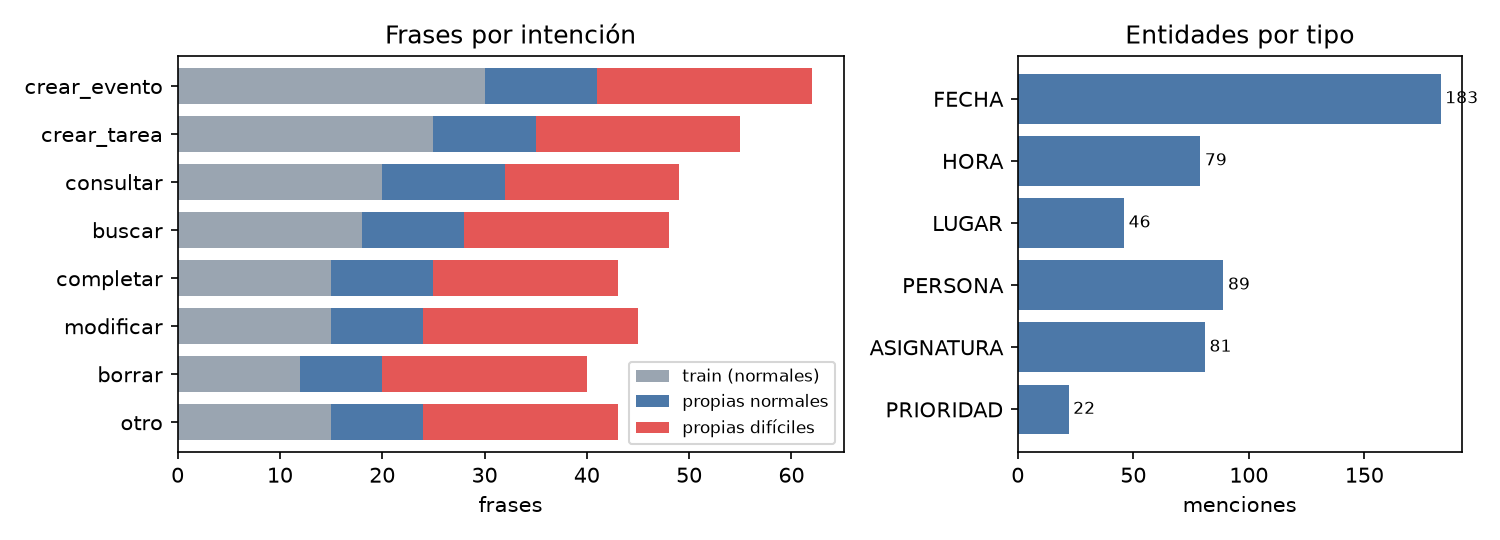
\includegraphics[width=\linewidth]{corpus.png}
  \caption{Corpus ampliado: frases por intención según origen y dificultad (izquierda) y menciones por tipo de entidad (derecha).}
  \label{fig:corpus}
\end{figure}

\begin{table}[h]
  \centering\small
  \begin{tabular}{@{}llr@{}}
    \toprule
    Tipo & Ejemplo & Frases \\
    \midrule
    abreviatura    & «q tngo pasado mñn» & 41 \\
    paráfrasis     & «Quita lo de los dientes» $\rightarrow$ Dentista & 22 \\
    fecha relativa & «dentro de tres días», «del 16 al 20» & 18 \\
    negación       & «No borres el dentista, solo muévelo a las 12» & 16 \\
    mayúsculas     & «QUÉ TENGO EL VIERNES» & 14 \\
    números en letras & «a las cuatro menos cuarto» & 12 \\
    ortografía     & «ya e pagao la matricula» & 10 \\
    fuera de dominio & «¿Qué tiempo hará el sábado?» & 10 \\
    larga          & 7 entidades en una frase & 9 \\
    contexto       & «Cena de empresa \dots{} a las 9» $\rightarrow$ 21:00 & 4 \\
    \midrule
    \multicolumn{2}{@{}l}{Total difíciles (normales: 79 propias + 150 de \cod{train})} & 156 \\
    \bottomrule
  \end{tabular}
  \caption{Tipos de dificultad de las frases propias.}
  \label{tab:dificultad}
\end{table}

\paragraph{Decisiones de etiquetado.} Donde el enunciado no fija la convención, seguimos lo que hace \cod{train.jsonl}: «antes del viernes» $\rightarrow$ FECHA = «del viernes»; en \cod{modificar}, «al viernes» $\rightarrow$ «viernes»; las franjas vagas («por la tarde») no son HORA; «en casa de mi madre» no es LUGAR; en PERSONA se anota el nombre propio o el parentesco sin posesivo («mi primo Dani» $\rightarrow$ «Dani»). Decisiones nuestras: en las fechas negadas («no es el miércoles, es el jueves») se anotan todas las menciones, porque B reconoce menciones y elegir el valor nuevo le corresponde al asistente; «del 16 al 20» se normaliza como el intervalo \cod{2026-02-16/2026-02-20}.
\pendiente{Revisión cruzada: número de discrepancias entre los dos integrantes y cómo se resolvieron.}

\paragraph{Análisis exploratorio.} El corpus tiene 3\,357 palabras y un vocabulario de 588 tipos (en minúsculas; TTR $=0{,}18$); el 45\,\% del vocabulario son hápax. La distribución sigue la ley de Zipf (pendiente log-log $-1{,}04$, figura~\ref{fig:zipf}), con la cola aplanada propia de un corpus pequeño: el test oculto traerá muchas palabras no vistas, lo que favorece los n-gramas de caracteres y los embeddings preentrenados. Con stopwords, las palabras más frecuentes (\textit{el, de, la, a}) son las mismas en todas las clases. Sin ellas aparecen los verbos que discriminan (\textit{borra/quita/elimina} en \cod{borrar}; \textit{cambia/mueve/pasa} en \cod{modificar}; \textit{urgente/prisa} en \cod{crear\_tarea}). Pero la lista de spaCy también elimina \textit{ya}, \textit{qué} y \textit{cuándo}, que caracterizan \cod{completar}, \cod{consultar} y \cod{buscar}. Las concordancias muestran que «mañana» es la FECHA ``día siguiente'' en 25 de sus 30 apariciones. El resto son la franja horaria («por la mañana») o frases \cod{otro}, que por convención no llevan entidades. Los días de la semana aparecen a menudo dentro de expresiones más largas («el jueves de la semana que viene» = 19), así que la normalización de fechas tiene que operar sobre la expresión completa. FECHA es el tipo dominante (183 de 500 entidades, figura~\ref{fig:corpus}), de modo que el F1 micro de B dependerá sobre todo de resolver bien las fechas. \cod{buscar}, \cod{completar} y \cod{borrar} apenas llevan entidades: la tarea C tiene que apoyarse en las palabras de contenido.

\begin{figure}[h]
  \centering
  \begin{minipage}[c]{0.46\linewidth}
    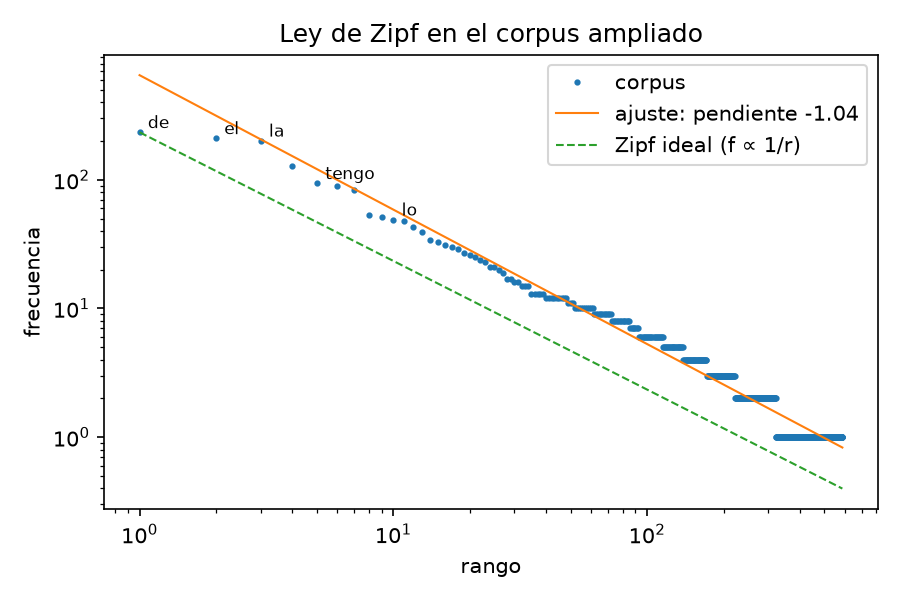
\includegraphics[width=\linewidth]{zipf.png}
    \captionof{figure}{Ley de Zipf en el corpus ampliado.}
    \label{fig:zipf}
  \end{minipage}\hfill
  \begin{minipage}[c]{0.5\linewidth}
    \centering\small
    \begin{tabular}{@{}lrrrr@{}}
      \toprule
      Tipo & TP & FP & FN & F1 \\
      \midrule
      PERSONA (PER) & 65 & 28 & 24 & 0,71 \\
      LUGAR (LOC)   & 5  & 12 & 41 & 0,16 \\
      \bottomrule
    \end{tabular}
    \captionof{table}{NER de spaCy (\cod{es\_core\_news\_md}) frente a nuestras etiquetas, comparando el texto normalizado como en \cod{evaluar.py}.}
    \label{tab:spacy}
  \end{minipage}
\end{figure}

\paragraph{Recursos lingüísticos (spaCy).} Con texto estándar, la tokenización, el POS y la lematización son correctos (\textit{tengo} $\rightarrow$ \textit{tener}, \textit{Javier} PROPN). Con lenguaje de mensajería, el modelo se rompe: en «q tngo mñn x la mñn» etiqueta todos los tokens como PROPN y propone «q tngo mñn x» como PER. Los clíticos también le fallan: \textit{márcalo} sale como PER y lematiza \textit{muévelo} como «muéveloir». En NER (tabla~\ref{tab:spacy}), spaCy solo tiene PER/LOC/ORG/MISC. PERSONA funciona razonablemente con nombres propios con mayúscula, pero se le escapan los parentescos («madre», «abuela») y los nombres en minúscula, y marca como persona verbos al principio de la frase («Tacha», «Adiós») y empresas («Indra»). LUGAR apenas funciona, porque nuestros lugares son nombres comunes con número («despacho 3204», «biblioteca») y no topónimos. Las asignaturas salen como ORG/MISC y no hay nada para FECHA, HORA ni PRIORIDAD. Conclusión para B2: spaCy para PERSONA completado con una lista de parentescos, y reglas para LUGAR y para el resto.

\paragraph{Preprocesado.} La función \cod{normalizar} (en \cod{utilidades.py}) es configurable:
\begin{itemize}
  \item minúsculas;
  \item tildes, conservando la ñ;
  \item diccionario de abreviaturas de mensajería (\textit{q, tngo, mñn, xq, bbdd}\dots);
  \item números escritos con letras («cinco» $\rightarrow$ 5; «una» solo en «la una»);
  \item stopwords de spaCy, excepto negaciones, interrogativos, palabras temporales y números;
  \item stemming Snowball o lematización con spaCy.
\end{itemize}
La tabla~\ref{tab:prepro} muestra que cada paso reduce la dispersión del vocabulario. Su efecto sobre los clasificadores se mide en E2 (sección~\ref{sec:experimentos}).

\begin{table}[h]
  \centering\small
  \begin{tabular}{@{}lrrl@{}}
    \toprule
    Configuración & Tokens & Vocabulario & «No borres el dentista, muévelo a la una» \\
    \midrule
    original                 & 3\,356 & 706 & No borres el dentista, muévelo a la una \\
    minúsculas + tildes      & 3\,356 & 569 & no borres el dentista, muevelo a la una \\
    + abreviaturas y números & 3\,374 & 551 & no borres el dentista , muévelo a la 1 \\
    + sin stopwords          & 1\,903 & 475 & no borres dentista , muévelo 1 \\
    + stemming               & 1\,903 & 387 & no borr dentist , muevel 1 \\
    \bottomrule
  \end{tabular}
  \caption{Efecto acumulado del preprocesado sobre el corpus.}
  \label{tab:prepro}
\end{table}

\paragraph{Partición.} \cod{train\_test\_split} con \cod{random\_state=0} y estratificación por \textbf{intención y dificultad}: 308 frases de entrenamiento y 77 de validación, de las que \textbf{31 son difíciles} (de 10 tipos distintos) y 36 tienen \cod{ref} (tarea C). Se guardan en \cod{mi\_train.jsonl} y \cod{mi\_validacion.jsonl} y no se regeneran.

% =====================================================================
\section{Enfoques}\label{sec:enfoques}
% Presupuesto: 1,5 páginas · Fases 2-4. Descripción breve y decisiones de diseño (sin repetir teoría).

\subsection{Tarea A · Intención}
Todos los enfoques están en \cod{tarea\_a.py}, y los entrenables son \textit{pipelines} de scikit-learn que incluyen su propio preprocesado (\cod{normalizar}), de modo que el modelo guardado en \cod{modelos/} se aplica directamente al texto crudo. Los hiperparámetros se eligen con validación cruzada estratificada de 5 particiones \textbf{sobre \cod{mi\_train}}; la validación solo se usa para medir.

\paragraph{A1 · Reglas.} 14 expresiones regulares sobre el texto en minúsculas, sin tildes y con las abreviaturas expandidas, aplicadas por prioridad: \cod{otro} evidente (el tiempo, fútbol, «recomiéndame»: frases con fechas y «cuándo» que no son de agenda) $\rightarrow$ \cod{borrar} (\textit{borr-, elimin-, quit-, cancel-}, tras quitar las negaciones «no borres») $\rightarrow$ \cod{completar} («ya\dots» sin «ya no», «he + participio», \textit{tacha}) $\rightarrow$ \cod{modificar} (\textit{cambi-, muev-, retras-}, «ahora es»; protegiendo «pasado mañana») $\rightarrow$ \cod{buscar} (\textit{cuándo, dónde, a qué hora}, «tenía») $\rightarrow$ \cod{consultar} («qué tengo», «estoy libre») $\rightarrow$ crear. Entre tarea y evento decide la hora («a las 5» $\rightarrow$ evento) y las marcas de tarea (\textit{tengo que, recuérdame, antes del, urgente}). Las órdenes explícitas («apunta», «recuérdame») desactivan las reglas de consulta y búsqueda.

\paragraph{A2 · BoW + Naive Bayes.} \cod{CountVectorizer} + \cod{MultinomialNB}. La validación cruzada elige texto normalizado, solo unigramas y $\alpha=0{,}1$ (los bigramas empeoran: con 308 frases casi todos son únicos).

\paragraph{A3 · TF-IDF + regresión logística.} Unión de TF-IDF de palabras (1--2-gramas) y de n-gramas de caracteres \cod{char\_wb} (2--4), con \textit{tf} sublineal y $C=10$. Los n-gramas de caracteres comparten subcadenas entre variantes con faltas o abreviaturas (\textit{bórralo/borra}, \textit{peluqeria}).

\paragraph{A4 · Word2Vec propio.} \textit{Skip-gram} de gensim (100 dimensiones, 50 épocas, \cod{workers=1} y semilla fija para que sea reproducible) entrenado solo con las frases de \cod{mi\_train}; cada frase es la media de sus vectores, seguida de regresión logística. Con unas 3\,000 palabras de entrenamiento los vectores no capturan semántica: las palabras más parecidas a \textit{borra} son \textit{han, juego, gano}.

\paragraph{A5 · Vectores preentrenados.} Media de los vectores de 300 dimensiones de \cod{es\_core\_news\_md} + regresión logística ($C=0{,}1$). Como los vectores son de palabras con tilde, el mejor preprocesado expande abreviaturas y números sin quitar tildes. Promediar solo las palabras de contenido (sin stopwords) empeora, como en E2.

\pendiente{Fase 3: A6 embeddings de frase + RL, A7 + RF/MLP, A8 LLM zero/few-shot.}

\subsection{Tarea B · Extracción}
\pendiente{Fase 4: normalización (\cod{normalizacion.py}), B1 reglas, B2 spaCy + reglas, B3 BETO + MLP/RF (BIO), B4 LLM con JSON.}

\subsection{Tarea C · Entrada referida}
\pendiente{Fase 4: documento de cada entrada, C1 palabras clave, C2 BM25/TF-IDF, C3 embeddings estáticos, C4 embeddings de frase, C5 híbrido (RRF), C6 re-ranking con LLM.}

% =====================================================================
\section{Tabla comparativa y discusión}\label{sec:tabla}
% Presupuesto: 2 páginas · Fases 2-5. Una fila por enfoque; columnas del enunciado.

\begin{table}[h]
  \centering\small
  \begin{tabular}{@{}lrrrrrrl@{}}
    \toprule
    Enfoque & F1 macro & Normales & Difíciles & Datos entr. & ms/frase & Tamaño & ¿Interpr.? \\
    \midrule
    A1 reglas                    & \textbf{0,908} & 0,953 & \textbf{0,845} & 0 (reglas) & 0,04 & 2 KB & sí \\
    A2 BoW + Naive Bayes         & 0,713 & 0,776 & 0,639 & 308 frases & 0,03 & 66 KB & sí \\
    A3 TF-IDF + RL               & 0,896 & \textbf{0,961} & 0,808 & 308 frases & 0,06 & 379 KB & parcial \\
    A4 Word2Vec propio + RL      & 0,607 & 0,619 & 0,581 & 308 frases & 0,04 & 205 KB & no \\
    A5 vectores spaCy + RL       & 0,843 & 0,889 & 0,771 & preentr. + 308 & 0,28 & 23 MB & no \\
    \bottomrule
  \end{tabular}
  \caption{Tarea A en validación (77 frases, 31 difíciles). El tamaño de A1 es el de sus expresiones regulares; el de A5 incluye la tabla de vectores de spaCy. \pendiente{fase 3: A6--A8.}}
  \label{tab:A}
\end{table}

\paragraph{Tarea A (fase 2).} Las reglas son el mejor enfoque clásico y el más robusto en frases difíciles, porque normalizan la mensajería antes de buscar los patrones. Pero en \cod{mi\_train}, donde se escribieron, sacan 0,991: una de cada diez frases nuevas ya se les escapa (paráfrasis como «Fuera lo del basket», «pásalo a\dots»). A3 casi empata sin escribir ninguna regla y es el mejor en frases normales; los n-gramas de caracteres son lo que lo separa de A2, que no generaliza a palabras no vistas. A5 demuestra que los vectores preentrenados sí aportan (0,843 frente a 0,607 de A4 con el mismo clasificador), a cambio de un modelo 60 veces mayor y más lento. Todos pierden entre 4 y 15 puntos en las frases difíciles.

\pendiente{Fase 5: tablas B y C, columnas manuales revisadas y comentario por tarea.}

% =====================================================================
\section{Experimentos}\label{sec:experimentos}
% Presupuesto: 3 páginas · Fases 2, 3 y 5.

\subsection{E1 · Curva de aprendizaje}
Entrenamos con 25, 50, 100 y las 308 frases de \cod{mi\_train} (submuestras estratificadas por intención, 5 semillas) y medimos en la validación completa (figura~\ref{fig:curva}). Las dos curvas siguen subiendo al llegar a las 308 frases, así que más datos seguirían ayudando. A3 va por delante en todos los tamaños y la distancia crece con los datos (0,05 con 25 frases, 0,18 con todas). Con unas 3 frases por intención ninguno pasa de 0,5, y ninguno alcanza a las reglas, que no necesitan datos.
\pendiente{Fase 3: añadir A6, A7 y la línea horizontal de A8; ¿a partir de cuántos ejemplos gana cada uno al LLM?}

\begin{figure}[h]
  \centering
  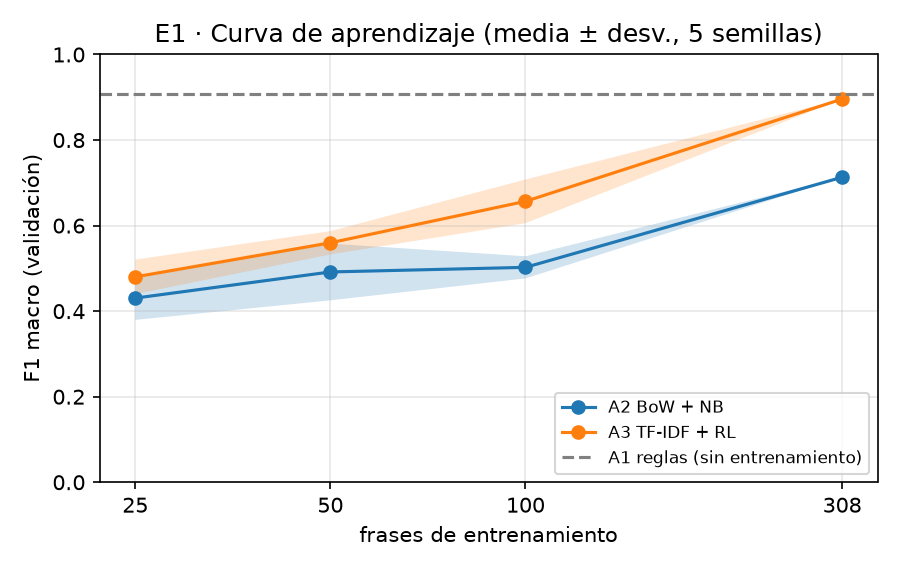
\includegraphics[width=0.62\linewidth]{curva_aprendizaje.png}
  \caption{E1: F1 macro en validación frente al número de frases de entrenamiento (media $\pm$ desviación de 5 semillas). Con todas las frases la desviación es 0 porque el conjunto es siempre el mismo.}
  \label{fig:curva}
\end{figure}

\subsection{E2 · Ablación del preprocesado}
\begin{table}[h]
  \centering\small
  \begin{tabular}{@{}lrrrr@{}}
    \toprule
    & \multicolumn{2}{c}{Todas (77)} & \multicolumn{2}{c}{Difíciles (31)} \\
    \cmidrule(lr){2-3}\cmidrule(l){4-5}
    Preprocesado & A2 & A3 & A2 & A3 \\
    \midrule
    original (sin cambios)                          & 0,700 & 0,841 & 0,512 & 0,802 \\
    normalizado (minúsc., tildes, abrev., números)  & \textbf{0,713} & \textbf{0,896} & \textbf{0,639} & 0,808 \\
    + sin stopwords                                 & 0,611 & 0,795 & 0,549 & \textbf{0,834} \\
    + stemming                                      & 0,576 & 0,805 & 0,494 & \textbf{0,834} \\
    \bottomrule
  \end{tabular}
  \caption{E2: F1 macro en validación según el preprocesado (configuraciones acumulativas). \pendiente{fase 3: columna A6.}}
  \label{tab:E2}
\end{table}

La normalización es la mejor configuración para los dos modelos de conteo (tabla~\ref{tab:E2}): une variantes de la misma palabra (\textit{mñn/mañana}, \textit{QUÉ/qué}) y reduce la dispersión, sobre todo en las frases difíciles de A2 (+0,13). Quitar stopwords \textbf{perjudica} ($-0{,}10$ en ambos): aunque conservamos \textit{no, ya, qué, cuándo}, la lista de spaCy quita \textit{lo, me, he, se}, que separan clases («lo de\dots» en \cod{borrar} y \cod{modificar}, «he pagado» en \cod{completar}). El stemming no recupera lo perdido. En las frases difíciles, A3 mejora sin stopwords (0,834), pero con 31 frases es una diferencia de una o dos frases.

\subsection{E3 · Robustez}
\pendiente{Fase 5: normales vs.\ difíciles para cada enfoque de A, B y C, desglosado por el campo \cod{dificultad}.}

\subsection{E4 · Análisis de errores}
\pendiente{Fase 5: $\geq$10 errores por familia agrupados por causa; mejora para la causa más frecuente con resultado antes/después.}

% =====================================================================
\section{Elección justificada por tarea}\label{sec:eleccion}
% Presupuesto: 1,5 páginas · Fase 5. Calidad, coste, latencia y riesgo.

\pendiente{Fase 5: un enfoque por tarea, con argumentos de calidad, coste, latencia y riesgo (alucinación, inyección de instrucciones, fragilidad de las reglas). Valorar híbridos.}

% =====================================================================
\section{El asistente}\label{sec:asistente}
% Presupuesto: 1 página · Fase 6.

\pendiente{Fase 6: arquitectura (A $\rightarrow$ B $\rightarrow$ C $\rightarrow$ acción), estado de diálogo, salvaguardas fuera del modelo, solapamientos, desambiguación y resultado de los 14 casos de la demo.}

% =====================================================================
\section{Limitaciones y trabajo futuro}\label{sec:limitaciones}
% Presupuesto: 1/2 página · se va completando en cada fase.

\begin{itemize}
  \item \textbf{Corpus pequeño y escrito por nosotros}: 385 frases, el 45\,\% del vocabulario son hápax y las frases difíciles las hemos escrito nosotros mismos, con el riesgo de que reflejen nuestro estilo y no el del test oculto.
  \item \textbf{Fecha fija}: todas las fechas relativas se resuelven respecto al 9-2-2026; algunas expresiones («el próximo martes», «el finde que viene») son ambiguas y las hemos evitado en el corpus.
  \item \textbf{Validación pequeña}: con 77 frases (31 difíciles), una frase mal clasificada mueve la F1 macro más de un punto; diferencias como la de A1 y A3 (0,012) no son significativas.
\end{itemize}
\pendiente{Fases 3-6: añadir las limitaciones que aparezcan.}

% =====================================================================
\section{Uso de IA generativa}\label{sec:ia}
% Presupuesto: 1/2 página.

\pendiente{A completar por el grupo.}

% =====================================================================
\section{Reproducibilidad}\label{sec:repro}
% Presupuesto: 1/4 página · se va completando en cada fase.

Python 3.12 con las versiones fijadas en \cod{requirements.txt} (spaCy 3.8 con \cod{es\_core\_news\_md} 3.8.0, scikit-learn 1.9, NLTK 3.10). Semilla \cod{random\_state=0} en la partición. Orden de ejecución: \cod{1\_corpus} $\rightarrow$ \cod{2A}, \cod{2B}, \cod{2C} $\rightarrow$ \cod{3\_evaluacion} $\rightarrow$ \cod{4\_asistente}. Las figuras de esta memoria se generan en los notebooks y se guardan en \cod{resultados/}.
Tarea A: validación cruzada con \cod{StratifiedKFold(5, shuffle=True, random\_state=0)}, \cod{random\_state=0} en las regresiones logísticas y Word2Vec con \cod{seed=0} y \cod{workers=1} (gensim 4.4), que da los mismos vectores en ejecuciones distintas. El enfoque elegido se guarda en \cod{modelos/tarea\_a.joblib} y lo carga \cod{tarea\_a.predecir\_intencion}.
\pendiente{Fases 3-6: semillas del resto de modelos, hardware y tiempos.}

\end{document}
